%\subsubsection{Klassediagrammer}
%Klassediagrammer anvendes som redskab til at designe og give overblik over de forskellige klasser. Hertil vil relationerne mellem de forskellige klasser blive tydeliggjort ved anvendelse af tilhørende symbolisering: nedarvning, association %aggregation, composition 
%med mere. Som det ses af \autoref{fig:klassediagram} beskrives hver klasse ud fra et unikt klassenavn, hvor der yderligere kan tildeles attributter og metoder til den givne klasse.\cite{Fowler2004} 

\subsubsection{Klassediagrammer}
Klassediagrammer anvendes som redskab til at beskrive strukturen i et givent system og dermed skabe overblik over forskellige klasser og relationer, der indgår i systemet. 

Som det ses af \autoref{fig:klassediagram} identificeres hver klasse ud fra et unikt klassenavn, hvor der yderligere kan tildeles attributter og metoder til klassen.

\begin{figure} [H]
\centering
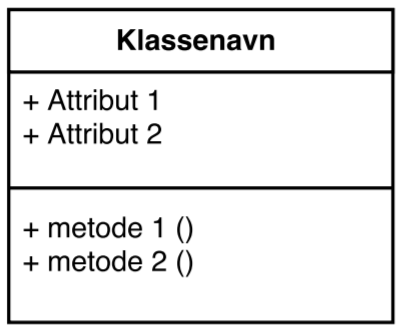
\includegraphics[width=0.5\textwidth]{figures/klassediag}
\caption{I klassediagrammer identificeres klasser ud fra et klassenavn, og dertilhørende attributter og metoder tilføjes nedenfor navnet.}
\label{fig:klassediagram}
\end{figure}

Attributter og metoder kan markeres med symbolerne; +, - eller #, som symboliserer, at de henholdsvis er public, private eller protected, jf. \autoref{sec:oop}.

Relationerne mellem klasserne illustreres ved brug af forskellige pile, og disse kan navngives for at tydeliggøre forholdet mellem  klasserne. Yderligere kan multipliciteten angives ved at tilføje symbolet *, der angiver "mange", eller specifikke værdier i pilenes ender. 















